%-------------------------------------------------------------------------------
\section{Methodology}
\label{methodology}
%-------------------------------------------------------------------------------
In this work, we focus narrowly on the class of failures for which traces of anomalous executions are \textit{structurally} deviate from traces of steady state executions. The assumption we make is that tracing accurately captures all causal interactions between system components both in the steady state execution as well as during the outage.

More generally, to reason about and compare executions after the fact, the assumption made is that attributes of interest such as memory or CPU usage and objects accessed for example, are captured.  Given this assumption, we can now assert that anomalous executions \textbf{must} deviate from steady state executions.

\begin{figure}[h]
\begin{center}
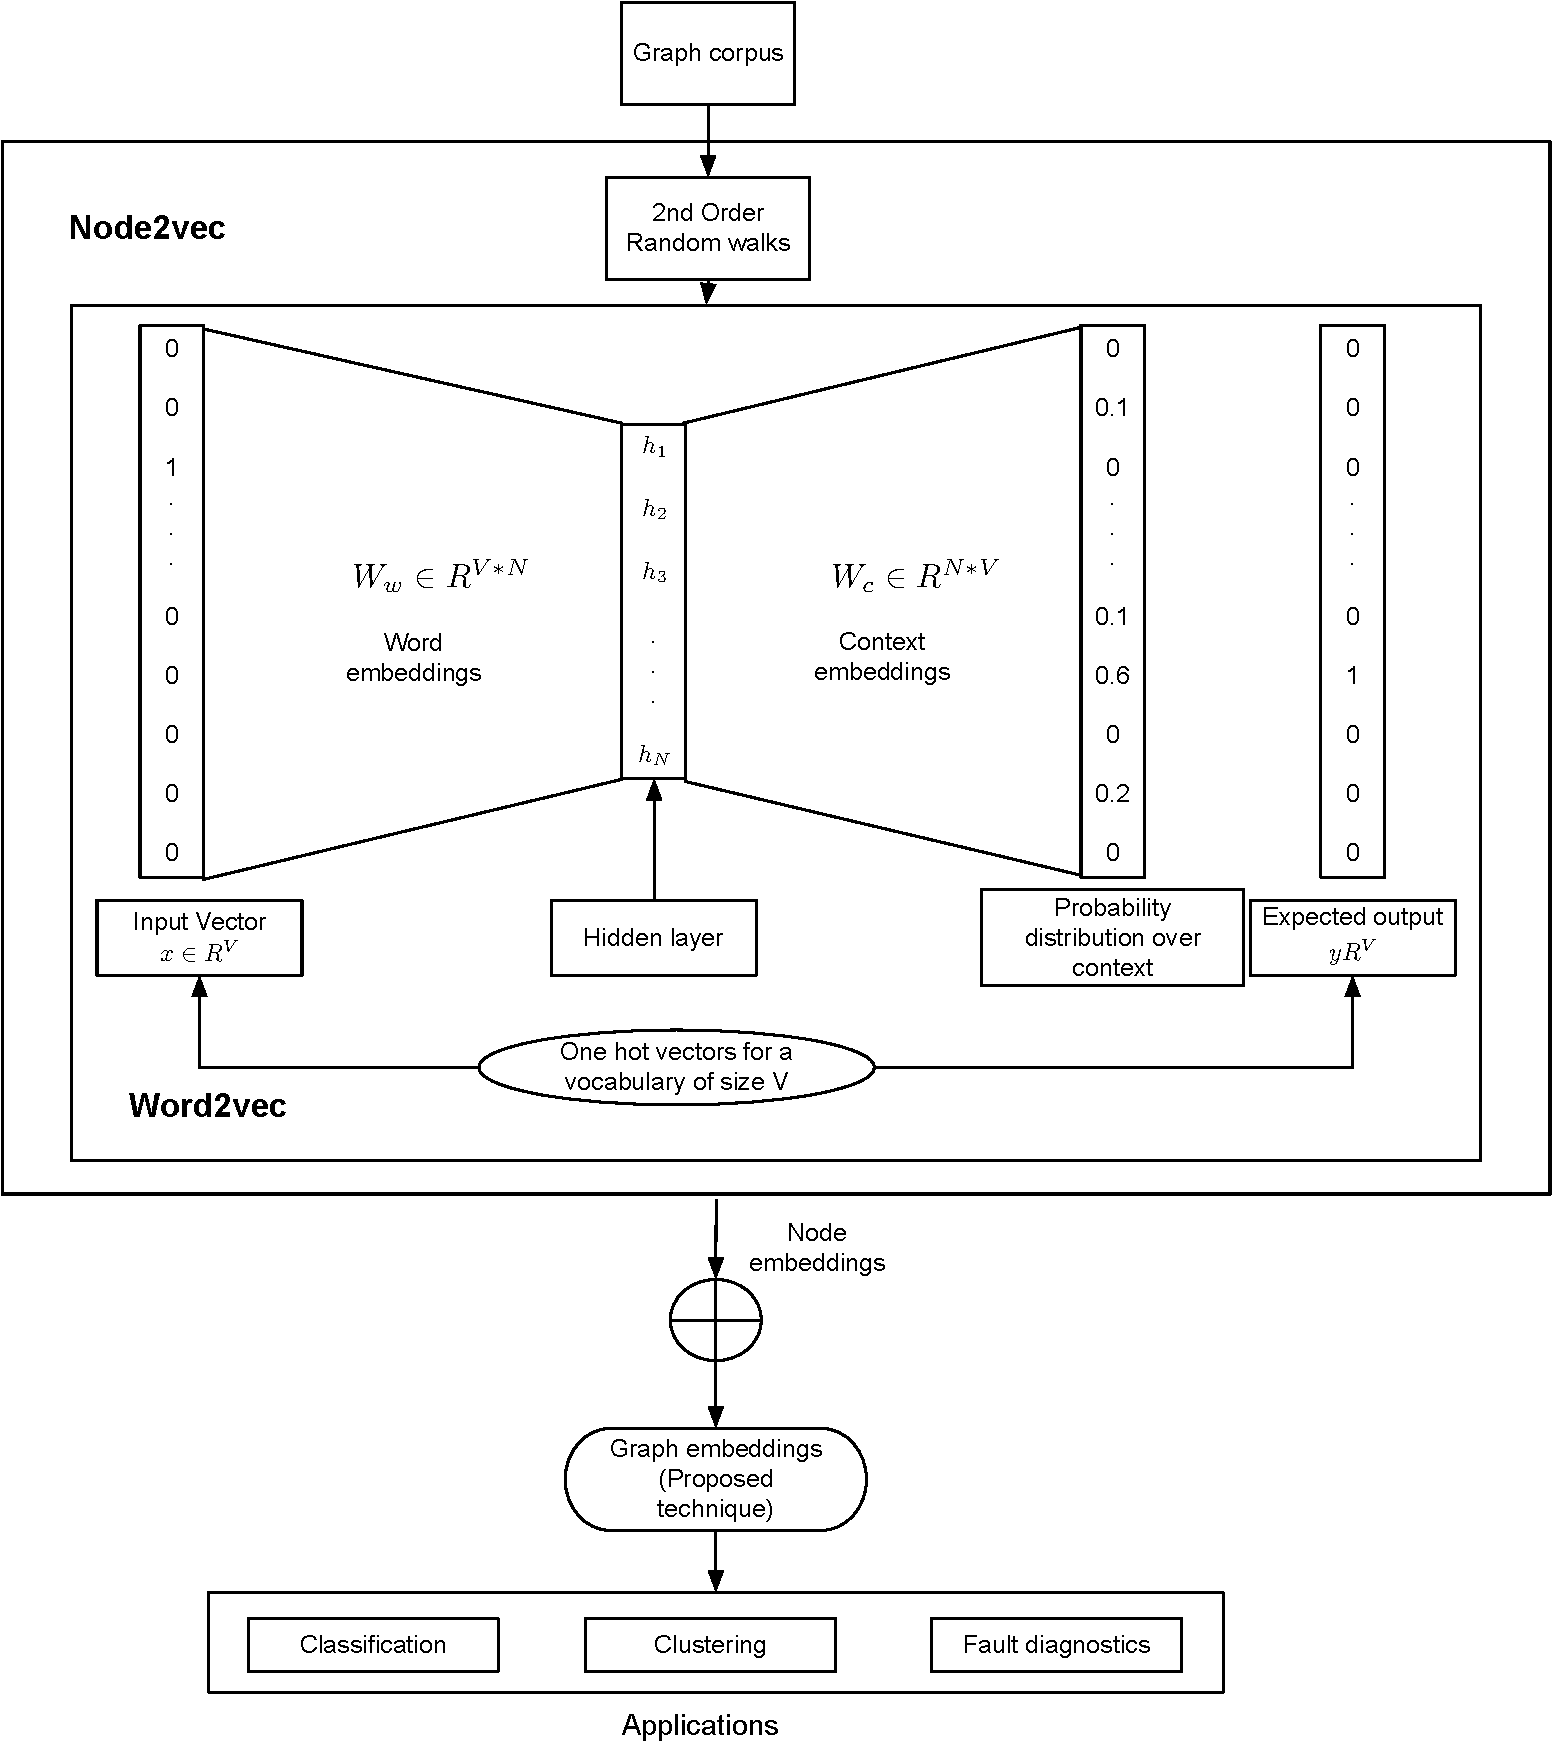
\includegraphics[width=0.4\textwidth, scale=0.25]{system_model.pdf}
\caption{System Model} 
\label{System_model}
\end{center}
\end{figure}

As can be seen in Figure~\ref{System_model}, our technique for generating trace representations derives from Word2Vec~\cite{Mikholv:2013:Word2vec}, popularly used to generate word embeddings based on context of words in a set of documents. We dub the learned trace representations as trace embeddings, which are fixed sized vectors in $R^{d}$ that capture the causal context of traces. We can now define appropriate distance measures to quantitatively compare pairs of traces with each other. 

%Embeddings serve two purposes:
%\begin{enumerate}
%\item Embeddings for traces can be classified before they are stored making it easy to find the most appropriate traces to compare to when a failure occurs.
%\item As the number as well as the size of traces increase, storing the embeddings may be much more compact than the original traces. \kam{Since we haven't tried reversing our embedding to recapture the graphs, there may be some information loss here which we will need to quantify while making this claim. If we want to make this claim, that is.}
%\end{enumerate}

Grover et al.~\cite{corr18_GroverL16} describe node2vec, which obtains node embeddings for graphs analogous to word embeddings obtained for documents. Graph nodes are considered words and random walks in the graph generate sentences for us to train on. As a result, the node embeddings encode information about its structural neighborhood. We use node2vec to obtain embeddings for trace events.

Our approach is to learn embeddings that encode structural information about the trace automatically from example traces.  We compute a trace embedding as an aggregate of embeddings of nodes in the graph corresponding to the trace, as this is the approach commonly taken in previous work~\cite{corr_2017_abs-1709-05584}. Of the various aggregator functions available such as summation, graph-coarsening approaches and graph neural networks, we chose summation for its simplicity and scalability. For precisely these reasons, it has been used in prior work~\cite{DBLP:journals/corr/DuvenaudMAGHAA15, DBLP:journals/corr/DaiDS16} to obtain subgraph embeddings. Intuitively, the resultant trace embedding is a linear combination of the component node embeddings. 

 Given trace embeddings and a distance measure, we evaluate the use of embeddings for generating hints to troubleshoot failures, for which we present qualitative results, as well as for clustering and classification that are typically needed to perform more complex tasks, for which we show quantitatively that our approach outperforms the state of the art which treats traces as bags of events.